% V2 - Sidebar. Tinted left panel (photo/contact/skills/education) + main column.
% Build: xelatex v2-sidebar.tex
\documentclass[10pt]{article}

\usepackage[a4paper, top=1.4cm, bottom=1.1cm, left=8.0cm, right=1.5cm]{geometry}
\usepackage{fontspec}
\usepackage{xcolor}
\usepackage{enumitem}
\usepackage{fontawesome5}
\usepackage{tikz}
\usepackage{eso-pic}
\usepackage[absolute,overlay]{textpos}
\usepackage[hidelinks]{hyperref}
\usepackage{microtype}
\usepackage{ragged2e}

\pagestyle{empty}
\setlength{\parindent}{0pt}
\linespread{1.0}
\setlength{\emergencystretch}{3em}

% ---- Fonts ----
\defaultfontfeatures{Path = /usr/share/fonts/rsms-inter-fonts/, Extension = .ttf, Ligatures = TeX}
\setmainfont{Inter}[UprightFont = Inter-Regular, BoldFont = Inter-SemiBold, ItalicFont = Inter-Italic]
\newfontfamily\interlight{Inter}[UprightFont = Inter-Light]
\newfontfamily\intermed{Inter}[UprightFont = Inter-Medium]
\newfontfamily\intersemi{Inter}[UprightFont = Inter-SemiBold]
\newfontfamily\displight{InterDisplay}[UprightFont = InterDisplay-Light]
\newfontfamily\dispthin{InterDisplay}[UprightFont = InterDisplay-Thin]

% ---- Palette ----
\definecolor{ink}{HTML}{20222A}
\definecolor{muted}{HTML}{767A85}
\definecolor{accent}{HTML}{1F5C63}     % deep teal
\definecolor{panel}{HTML}{EFEEEA}      % warm light grey
\definecolor{panelink}{HTML}{2A2C33}
\definecolor{hair}{HTML}{D6D7DB}
\color{ink}

\setlist[itemize]{leftmargin=1.05em, itemsep=0.25ex, topsep=0.4ex, parsep=0pt,
  label=\textcolor{accent}{\fontsize{5}{5}\selectfont\faSquare}}

% ---- Sidebar full-height panel on every page ----
\AddToShipoutPictureBG{\AtPageLowerLeft{\color{panel}\rule{7.0cm}{\paperheight}}}

% ---- Macros ----
\newcommand{\mainsec}[1]{\vspace{1.6ex}{\intersemi\footnotesize\addfontfeature{LetterSpace=14.0}\textcolor{accent}{\MakeUppercase{#1}}}\hspace{0.8em}\raisebox{0.28ex}{\textcolor{hair}{\leaders\hrule height 0.5pt\hfill\kern0pt}}\par\vspace{0.9ex}}
\newcommand{\sidesec}[1]{\vspace{2.6ex}{\intersemi\scriptsize\addfontfeature{LetterSpace=18.0}\textcolor{accent}{\MakeUppercase{#1}}}\par\vspace{0.4ex}{\color{hair}\hrule height 0.5pt}\vspace{1.0ex}}
% #1 title (short — keeps the date on the same line), #2 dates, #3 org + subtitle
\newcommand{\role}[3]{{\intersemi #1}\hfill{\scriptsize\textcolor{muted}{\mbox{#2}}}\par\vspace{0.3ex}{\small #3}\par\vspace{0.7ex}}
\newcommand{\skillgroup}[2]{{\intersemi\small #1}\par\vspace{0.3ex}{\small\textcolor{panelink}{#2}}\par\vspace{1.5ex}}
\newcommand{\contactline}[2]{\par\vspace{0.85ex}\noindent\makebox[1.5em][l]{\textcolor{accent}{#1}}\parbox[t]{\dimexpr\linewidth-1.5em\relax}{\RaggedRight #2}}

\begin{document}

% ===================== SIDEBAR =====================
\begin{textblock*}{5.5cm}(0.85cm,1.25cm)
  \color{panelink}
  \centering
  \begin{tikzpicture}
    \clip (0,0) circle (1.7cm);
    \node at (0,0) {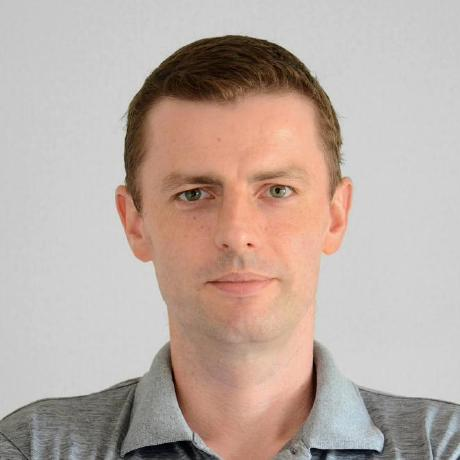
\includegraphics[width=3.6cm]{Profile-headshot-colour.png}};
    \draw[hair, line width=1.1pt] (0,0) circle (1.69cm);
  \end{tikzpicture}\par
  \vspace{0.5ex}
  \raggedright
  \sidesec{Contact}
  {\small
  \contactline{\faMapMarker*}{Osaka, Japan}
  \contactline{\faEnvelope[regular]}{\href{mailto:markhedleyjones@gmail.com}{markhedleyjones@gmail.com}}
  \contactline{\faGlobe}{\href{https://markhedleyjones.com}{markhedleyjones.com}}
  \contactline{\faGithub}{\href{https://github.com/markhedleyjones}{github.com/markhedleyjones}}
  \contactline{\faOrcid}{\href{https://orcid.org/0000-0003-3387-2932}{0000-0003-3387-2932}}}

  \sidesec{Skills}
  \skillgroup{Robotics \& Perception}{ROS, SLAM, 3D mapping, point clouds, object detection \& tracking}
  \skillgroup{Vision \& Machine Learning}{OpenCV, PyTorch, OpenVINO, sensor fusion}
  {\intersemi\small Software}\hfill{\small\textcolor{muted}{10+~years}}\par\vspace{0.3ex}{\small\textcolor{panelink}{C/C++, Python, Linux, Docker}}\par\vspace{1.5ex}
  \skillgroup{Design \& Fabrication}{SolidWorks, CAD/CAM, CNC, PCB \& embedded}

  \sidesec{Education}
  \skillgroup{Doctor of Philosophy}{University of Waikato, 2011–2015}
  \skillgroup{Master of Engineering}{First class honours, 2009}
  \skillgroup{Bachelor of Science}{Electronics \& mechatronics, 2005–2008}

  \sidesec{Awards}
  {\small\color{panelink}%
  Waikato Doctoral Scholarship \textcolor{muted}{(2010)}\par\vspace{0.45ex}
  Agilent Research Scholarship \textcolor{muted}{(2009)}\par\vspace{0.45ex}
  ENZcon Best Research Paper \textcolor{muted}{(2011)}\par\vspace{0.45ex}
  ENZcon Runner-up Presentation \textcolor{muted}{(2014)}\par}

  \sidesec{Languages \& Status}
  \skillgroup{Languages}{English (native), Japanese (conversational, JLPT N3)}
  \skillgroup{Nationalities}{New Zealand \& British}
  \skillgroup{Residency}{Japan (permanent resident)}
\end{textblock*}

% ===================== MAIN =====================
\RaggedRight
{\dispthin\fontsize{31}{34}\selectfont\addfontfeature{LetterSpace=2.0} Mark Hedley Jones}\par
\vspace{1.2ex}
{\intermed\large\textcolor{accent}{Robotics Perception Engineer}}\par
\vspace{0.6ex}
{\interlight\textcolor{muted}{SLAM \ \textbullet\ \ 3D mapping \ \textbullet\ \ sensor fusion}}

\mainsec{Profile}
{\interlight Over a decade building and shipping autonomous robots, from research platforms to deployed commercial fleets. PhD-qualified, spanning perception software, mechanical design and embedded hardware, with an AI-native workflow.}

\mainsec{Experience}
\role{Software Engineer}{Nov 2018 — Present}{\textcolor{accent}{SEQSENSE, Tokyo} \interlight\textcolor{muted}{— mapping, simulation \& object detection}}
Perception and mapping software for SEQSENSE's autonomous robots: \textbf{SQ-2}, a security robot deployed as a fleet across airports, offices and public buildings in Japan, and \textbf{FORRO}, a delivery robot co-developed with Kawasaki Heavy Industries.
\begin{itemize}
  \item On-line lidar-based 3D mapping (point clouds / PCD) across desktop, cloud and on-robot in real time.
  \item 3D object detection and tracking from lidar and camera; models trained in \textbf{PyTorch} and \textbf{OpenVINO}.
  \item \textbf{Gazebo} simulation mirroring robot behaviour; robot models (\textbf{URDF}) from CAD.
\end{itemize}

\vspace{0.8ex}
\role{Post-Doctoral Researcher}{Dec 2017 — Oct 2018}{\textcolor{accent}{Robotics Plus / University of Auckland} \interlight\textcolor{muted}{— autonomous navigation}}
Navigation software for heavy-duty vehicles in outdoor orchards.
\begin{itemize}
  \item Integrated and tuned real-time \textbf{SLAM}, point-cloud processing and path-planning; fused lidar, cameras, radar, IMU and GNSS.
  \item Personally accountable for the safety of people and infrastructure around the autonomous vehicle.
\end{itemize}

\vspace{0.8ex}
\role{Post-Doctoral Researcher}{Mar 2015 — Dec 2017}{\textcolor{accent}{Robotics Plus / University of Waikato} \interlight\textcolor{muted}{— robotic hardware development}}
Designed and built a heavy-duty outdoor vehicle, a fruit-harvesting robot and a pollination robot; led the research team.
\begin{itemize}
  \item Built \textbf{ROS} systems for robotic arms, precision spraying and an electric vehicle; full hardware design and integration.
  \item Managed a 6–10 person team across two universities, with budget and procurement authority.
\end{itemize}

\mainsec{Selected Publications}
\begin{itemize}
  \item \textbf{Jones, M.\,H.}, et al. \textit{Design and Testing of a Heavy-Duty Platform for Autonomous Navigation in Kiwifruit Orchards.} Biosystems Engineering, 2019.
  \item \textbf{Jones, M.\,H.}, Scott, J. \textit{Scaling of Electrode–Electrolyte Interface Model Parameters in Phosphate Buffered Saline.} IEEE Trans. Biomedical Circuits \& Systems, 2014.
  \item Williams, H., et al. (incl.\ \textbf{Jones, M.\,H.}). \textit{Large-scale evaluation of a robotic kiwifruit harvester.} Journal of Field Robotics, 2019.
\end{itemize}
{\small\textcolor{muted}{Full list \textbullet\ \href{https://markhedleyjones.com/about}{markhedleyjones.com/about}}}

\mainsec{Open Source \& Tools}
{\textbf{Container-Magic}, \textbf{dmenu-extended}, \textbf{Blender PCD I/O} \textcolor{muted}{— reproducible containerised dev environments and Linux/3D utilities}. \textbf{Calibration checkerboard collection} \textcolor{muted}{— widely used across the robotics \& CV community}.}

\end{document}
